\section{Experiments}
\label{sec:experiments}


\subsection{Experimental Setup}
\textbf{Datasets.} We conduct our state-of-the-art comparisons and ablation experiments on the KITTI-360 dataset \cite{liao2022kitti}. 
KITTI-360 contains images and LiDAR scans collected with a 64-beam LiDAR sensor across suburban areas of Karlsruhe, Germany, comprising approximately 80k scans from 9 sequences. 
For LiDAR scene generation, we follow the standard dataset split used in prior works \cite{zyrianov2022learning, nakashima_lidar_2024, nakashima_fast_2025}.  

To pretrain the flow matching (FM) model, we use ImageNet-1k \cite{liao2022kitti}, which contains over 1 million images.

\textbf{Implementation Details.}
We use 3D self-supervised features from ScaLR \cite{puy2024three}, which ranks among the state-of-the-art self-supervised backbones for LiDAR.
We implement our FM model using the base Scalable Interpolant Transformer~\cite{ma_sit_2024} with a patch size of 2 (SiT-B/2).
We train SiT-B/2 for 1M steps with a batch size of 256 using the Stable Diffusion VAE on ImageNet, following the official code and protocol of \cite{leng_repa-e_2025}.
During the VAE alignment stage, we train our VAE from scratch for 800k steps with a batch size of 32. After alignment, we perform end-to-end training for 1M steps, also with a batch size of 32. 
We set $\lambda_1$ and $\lambda_2$ to 1.5 and 0.5, respectively, as in \cite{wang_repa_2025}.
 
\textbf{Metrics.}  We evaluate the distance between the distributions of real and generated scenes using the Fr\'echet distance computed on different feature representations. 
Following \cite{ran_towards_2024}, we report Fr\'echet Range Image Distance (FRID), Fr\'echet Sparse Volume Distance (FSVD), and Fr\'echet Point Volume Distance (FPVD). 
In addition, we introduce Fréchet Localization Distance (FLD) to assess the quality of range images. 

LiDM \cite{ran_towards_2024} computes FRID using RangeNet++ \cite{milioto_rangenet_2019} trained on SemanticKITTI \cite{behley2019iccv}. 
However, we observed that FRID scores using RangeNet++ were not correlated with qualitative results, yielding unrealistically good scores for geometrically corrupted inputs. Our analysis shows that the model fails to segment KITTI-360 scenes, due to resolution differences: SemanticKITTI range images are twice as wide as those in KITTI-360. To address this, we replace RangeNet++ with RangeViT \cite{ando_rangevit_2023}, trained on SemanticKITTI range images whose spatial dimensions match those of KITTI-360. 

FSVD and FPVD are computed directly in the point cloud space using the LiDAR segmentation models MinkowskiNet \cite{choy2019minknet} and SPVCNN \cite{spvnas}, respectively. 
We argue that these metrics provide a more reliable measure of generation quality, as they operate directly on the point cloud and are not affected by projection discrepancies.

FLD is computed using the LIP-Loc model \cite{puligilla_lip-loc_2024}, which is trained in a CLIP-like manner for cross-modal localization between range images and camera images.

In addition to perceptual metrics, we compare the histograms of the bird’s-eye view point distribution using Jensen–Shannon Divergence (JSD). 
Finally, we compute the Minimum Matching Distance (MMD) \cite{ran_towards_2024}, which measures the Chamfer distance between each validation bird's-eye view voxelized scene and its closest generated counterpart.

\subsection{Comparison to state-of-the-art}
\newcommand\tabsetting{
\newcommand\rf[2]{\,{\scriptsize ##1\,'##2}}
}
\begin{table*}[htbp]


\caption{Quantitative Comparison of Unconditional Generation on KITTI-360.} 
\vspace{-0.2cm}
\label{tab:sota}
\centering
\tabsetting
\small
\resizebox{\linewidth}{!}{%

\begin{tabular}{lcccccccccccc}  
\toprule

&  &  \multicolumn{5}{c}{\textbf{Train-val}}  &  \multicolumn{5}{c}{\textbf{Val-only}} &  \\
\cmidrule(lr){3-7} \cmidrule(lr){8-12} 
 
 \multicolumn{1}{l}{\rotatebox{0}{\textbf{Method}}}   
  & \multicolumn{1}{c}{\textbf{Reference}}    
 & \multicolumn{1}{c}{\textbf{FRID}}    
 & \multicolumn{1}{c}{\textbf{FLD}}  
 & \multicolumn{1}{c}{\textbf{FSVD}}  
 & \multicolumn{1}{c}{\textbf{FPVD}}  
 & \multicolumn{1}{c}{\textbf{JSD}}    
   
 & \multicolumn{1}{c}{\textbf{FRID}}    
 & \multicolumn{1}{c}{\textbf{FLD}}  
 & \multicolumn{1}{c}{\textbf{FSVD}}  
 & \multicolumn{1}{c}{\textbf{FPVD}}  
 & \multicolumn{1}{c}{\textbf{JSD}}    
 % & \multicolumn{1}{c}{\textbf{TV}} 
 & \multicolumn{1}{c}{\textbf{MMD}}  
 \\
   & & {\footnotesize $\times 10^{0}$} & {\footnotesize $\times 10^{-1}$}  & {\footnotesize $\times 10^{0}$} & 
{\footnotesize $\times 10^{0}$} & {\footnotesize $\times 10^{-2}$}  & {\footnotesize $\times 10^{0}$} & {\footnotesize $\times 10^{-1}$} & {\footnotesize $\times 10^{0}$} & {\footnotesize $\times 10^{0}$} & {\footnotesize $\times 10^{-2}$} & {\footnotesize $\times 10^{-5}$}\\
 \midrule

UltraLiDAR & \cite{xiong_ultralidar_2023}\rf{cvpr}{23}  & - & - & 71.69 & 64.78 & 74.72  & - & - & 73.59 & 65.83 & 74.72 &  123.30 \\

LiDM & \cite{ran_towards_2024}\rf{cvpr}{24}  & 42.31 & 9.52 & 16.54 & 17.60 & 18.87  & 47.33 & 10.19 & 16.01 & 17.36 & 19.17 &  11.32 \\

LiDM w/ APE& \cite{ran_towards_2024}\rf{cvpr}{24}  & 37.01 & 6.12 & 13.79 & 13.82 & 11.24  & 42.09 & 9.76 & 13.68 & 13.86 & 11.69 &  9.95 \\

R2DM  & \cite{nakashima_lidar_2024}\rf{icra}{24}      & 9.84 & 4.04 & \underline{10.99} & \underline{11.99} & \underline{4.97}  &  15.54 & \underline{7.89} & \underline{12.67} & \underline{13.21} & \underline{5.78}  & \underline{8.50} \\

R2Flow   & \cite{nakashima_fast_2025}\rf{icra}{25}   & \textbf{3.89} & \underline{3.82} & 18.48 & 18.53 & 5.17  & \underline{8.87} & 8.36 & 20.80 & 20.27 & 5.97 &  \textbf{7.84}  \\
\midrule
\textbf{\ours} & ours & \underline{4.11} & \textbf{2.06} & \textbf{7.76} & \textbf{9.39} & \textbf{4.84} & \textbf{8.46} & \textbf{6.34} & \textbf{9.83} & \textbf{11.00} & \textbf{5.67}  & 8.72 \\

\bottomrule
\end{tabular}
}

\begin{tablenotes}[para]
    %\item 
    \footnotesize Best results are shown in \textbf{bold}, and second-best results are \underline{underlined}. FRID and FLD measure generation quality in the range image level, FSVD and FPVD in the point-cloud space, and JSD and MMD in the bird’s-eye view. APE stands for Absolute Positional Encoding.
\end{tablenotes}

\end{table*}



\begin{figure*}[t!]
    \centering
    \begin{tabular}{cccc}
        % Column 1
        \begin{minipage}{0.22\textwidth}
            \centering
            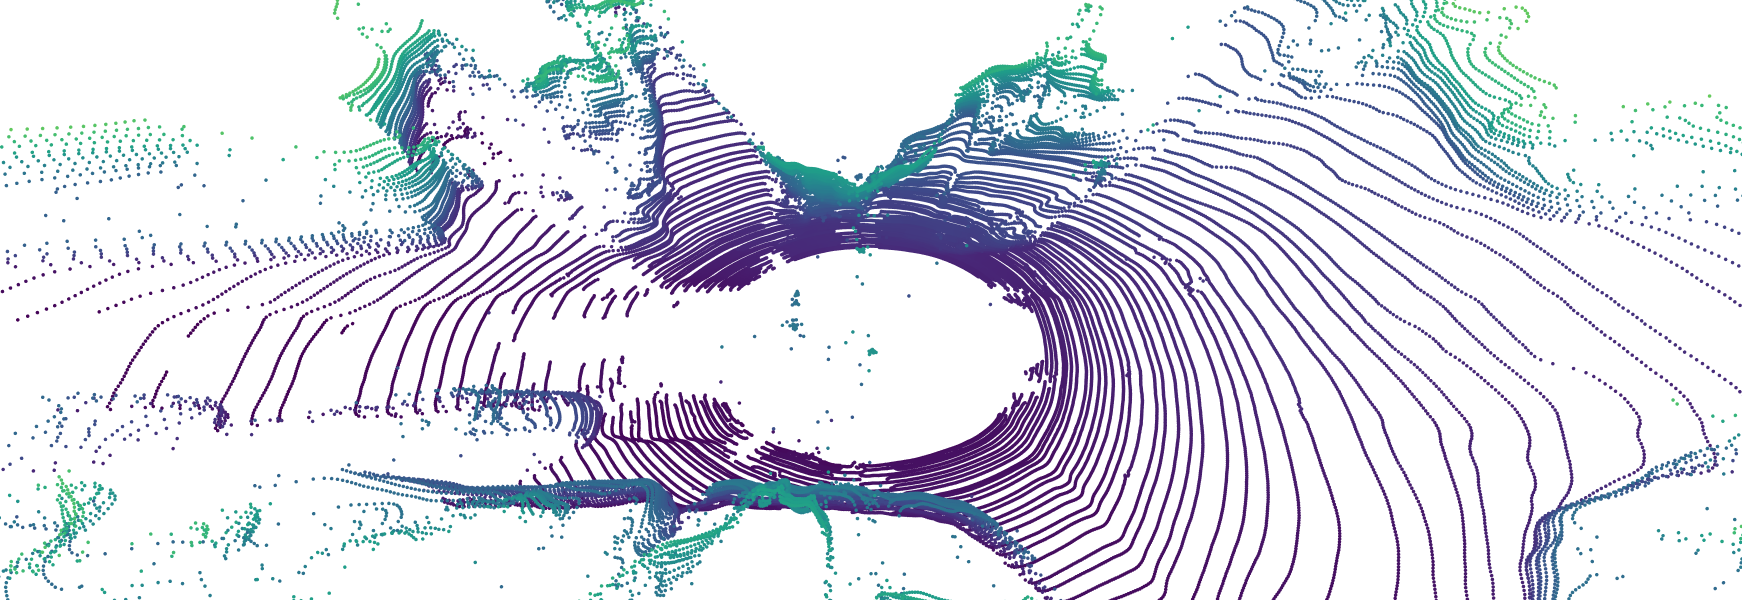
\includegraphics[width=\linewidth]{figures/pc_visu/lidm/lidm1.png} \\[0.5ex]
            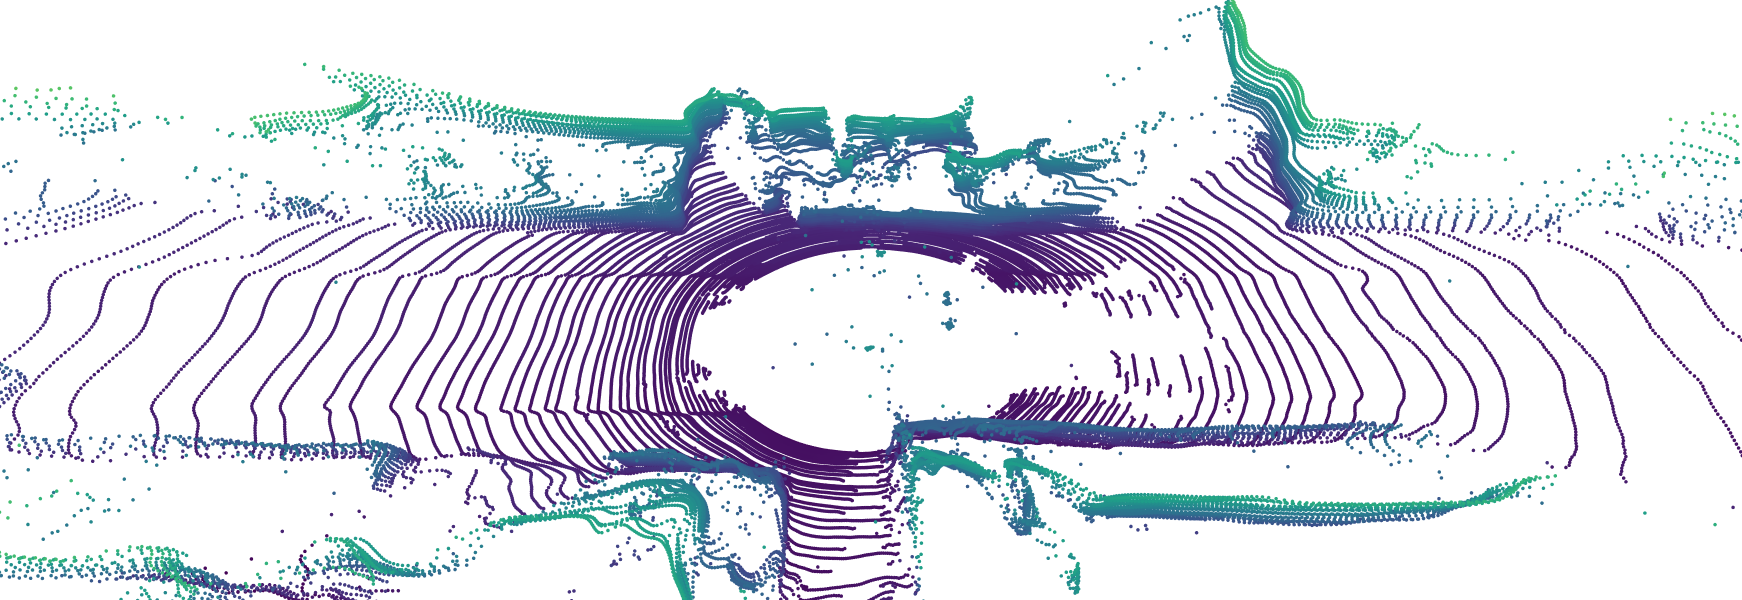
\includegraphics[width=\linewidth]{figures/pc_visu/lidm/lidm2.png} \\[0.5ex]
            \small{LiDM~\cite{ran_towards_2024}}
        \end{minipage} &
        % Column 2
        \begin{minipage}{0.22\textwidth}
            \centering
            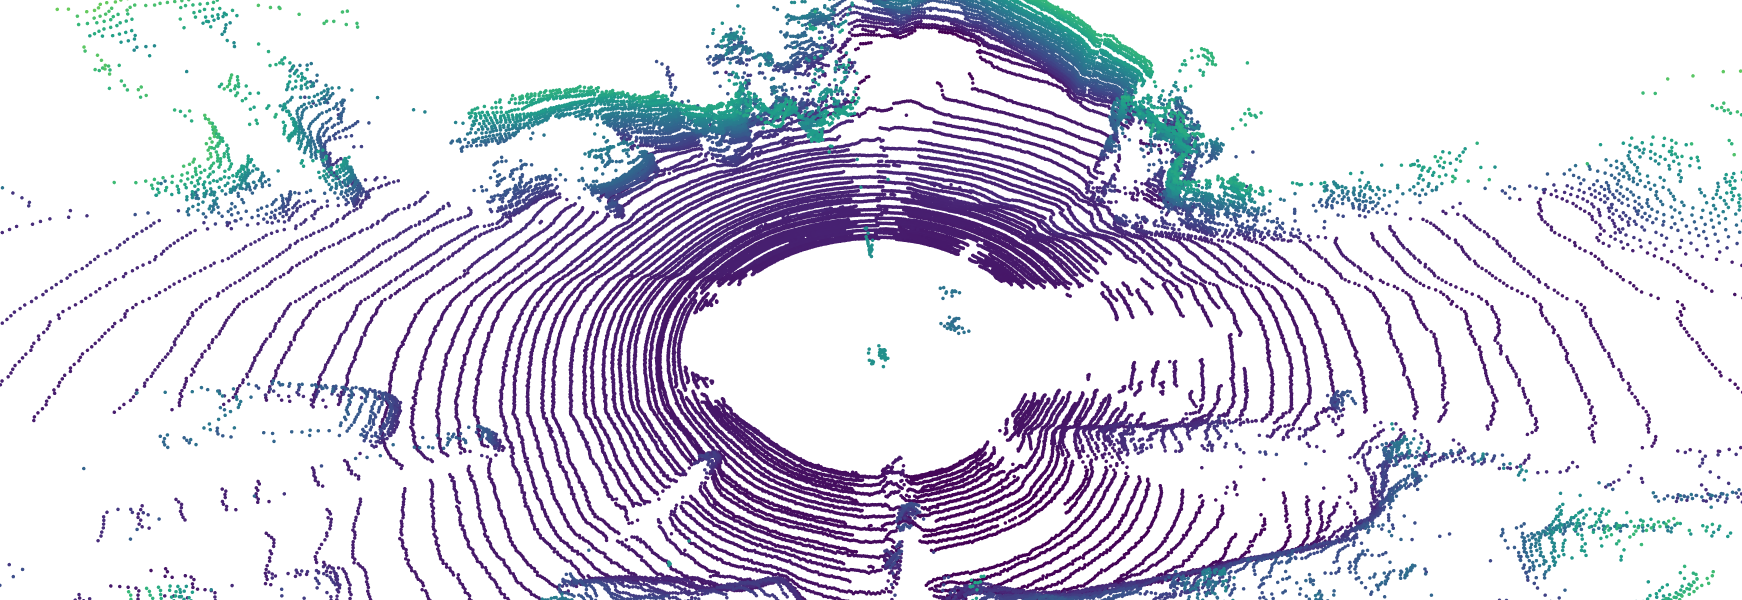
\includegraphics[width=\linewidth]{figures/pc_visu/r2dm/r2dm1.png} \\[0.5ex]
            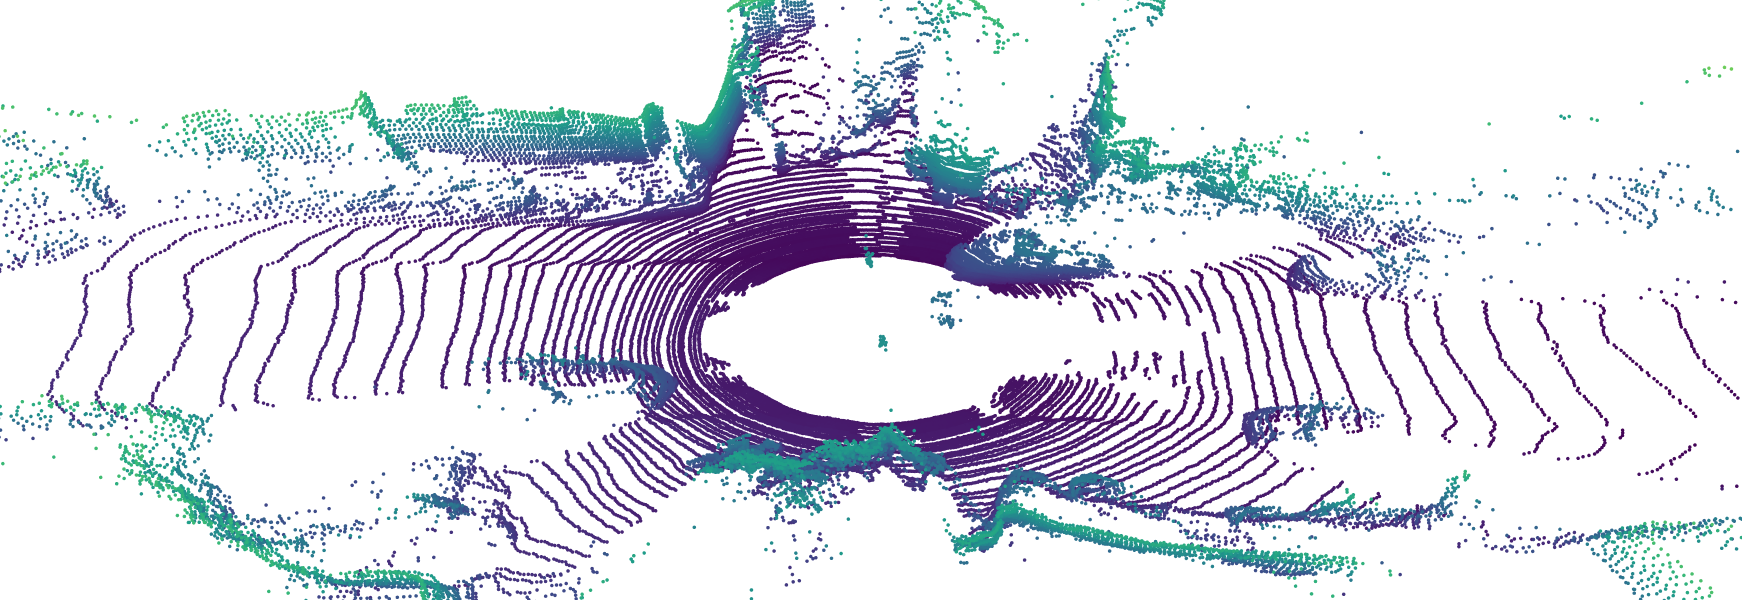
\includegraphics[width=\linewidth]{figures/pc_visu/r2dm/r2dm2.png} \\[0.5ex]
            \small{R2DM~\cite{nakashima_lidar_2024}}
        \end{minipage} &
        % Column 3
        \begin{minipage}{0.22\textwidth}
            \centering
            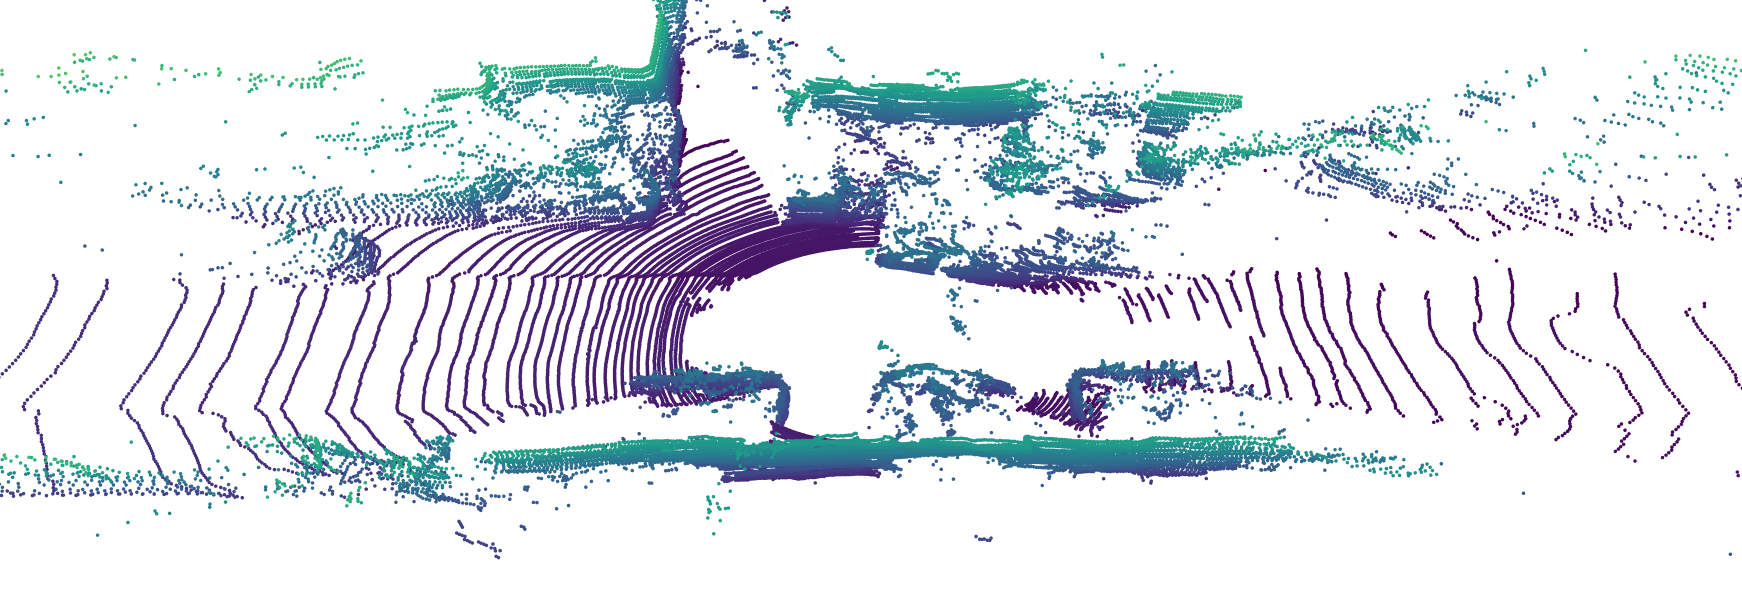
\includegraphics[width=\linewidth]{figures/pc_visu/r2flow/r2flow1.png} \\[0.5ex]
            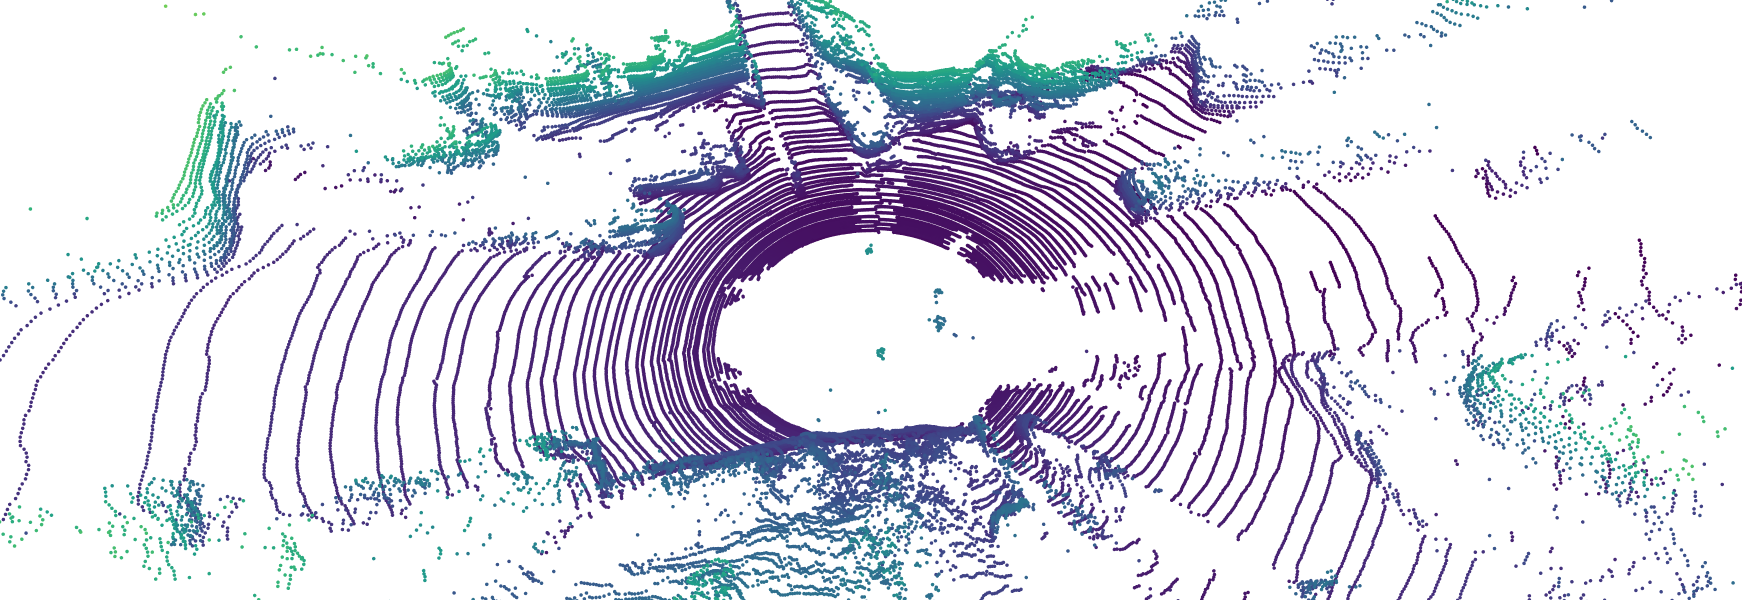
\includegraphics[width=\linewidth]{figures/pc_visu/r2flow/r2flow2.png} \\[0.5ex]
            \small{R2Flow~\cite{nakashima_fast_2025}}
        \end{minipage} &
        % Column 4
        \begin{minipage}{0.22\textwidth}
            \centering
            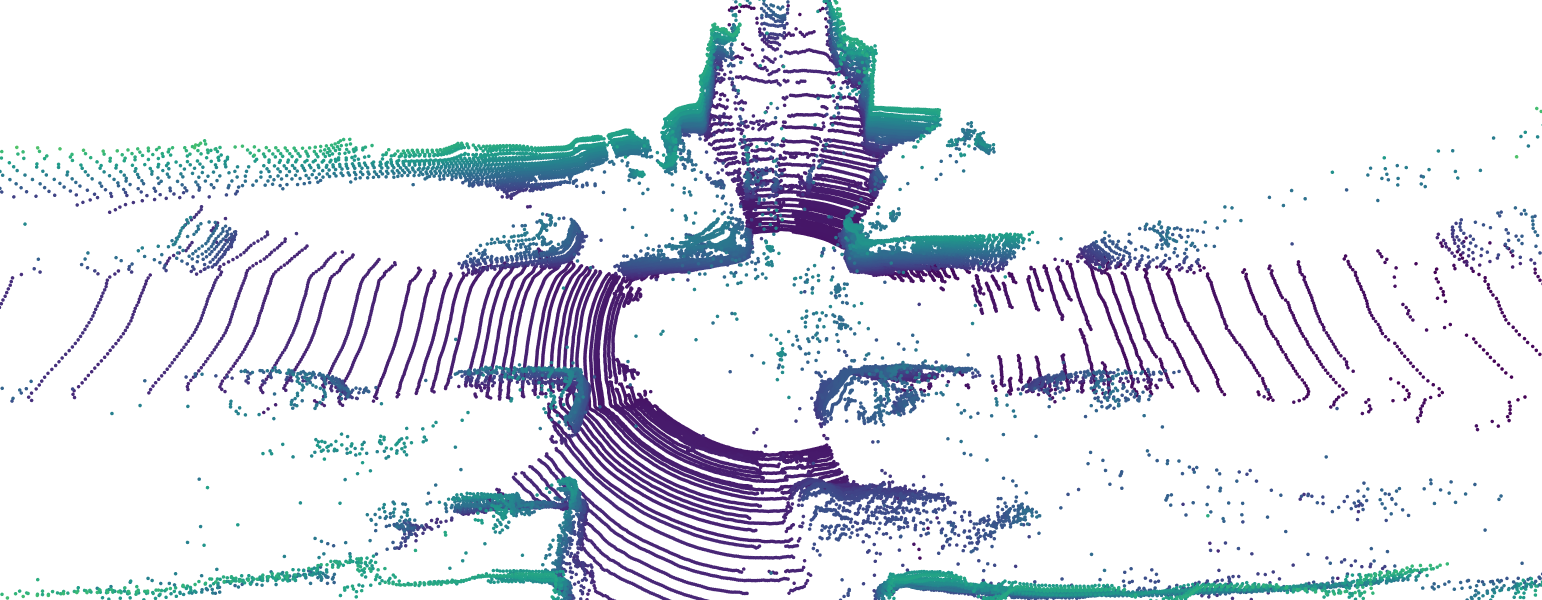
\includegraphics[width=\linewidth]{figures/pc_visu/r3dpa/r3dpa1.png} \\[0.5ex]
            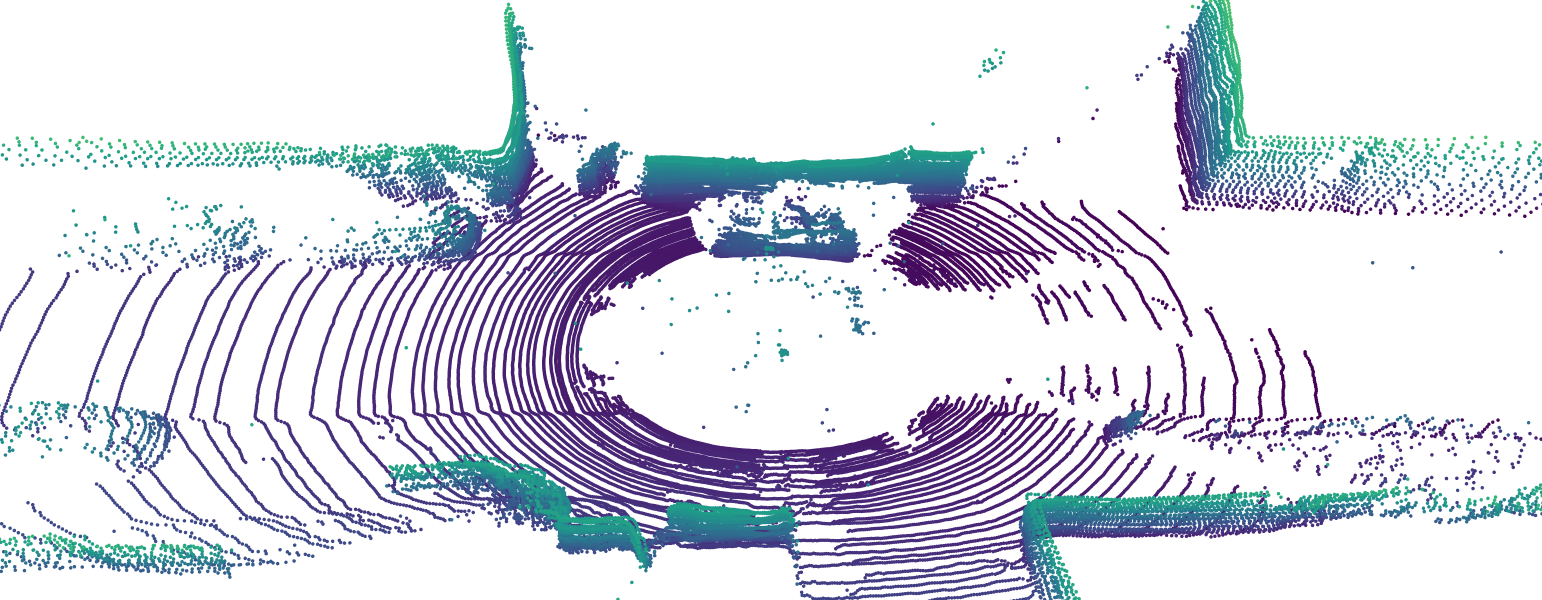
\includegraphics[width=\linewidth]{figures/pc_visu/r3dpa/r3dpa2.png} \\[0.5ex]
            \small{\textbf{\ours}}
        \end{minipage} \\
    \end{tabular}
    \caption{\textbf{Qualitative comparison of unconditional generations.} Our model generates high-quality point clouds with diverse and realistic objects.}
    \label{fig:qual}
\end{figure*}

%%%%%%%%%%%%%%%%%%%%%%
% \begin{figure*}
%     \centering
%     \begin{minipage}{0.24\textwidth}
%     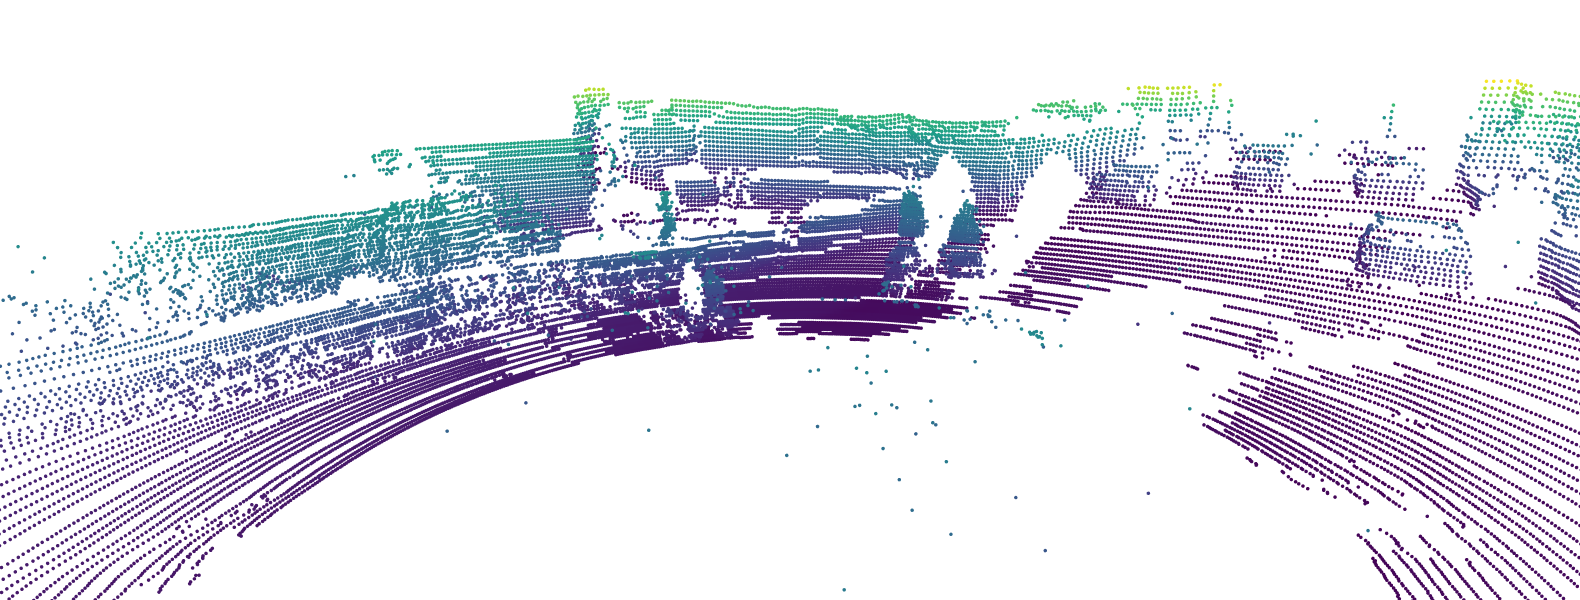
\includegraphics[width=\linewidth]{figures/qualitative/q1.png}
%     \end{minipage}
%     \begin{minipage}{0.24\textwidth}
%     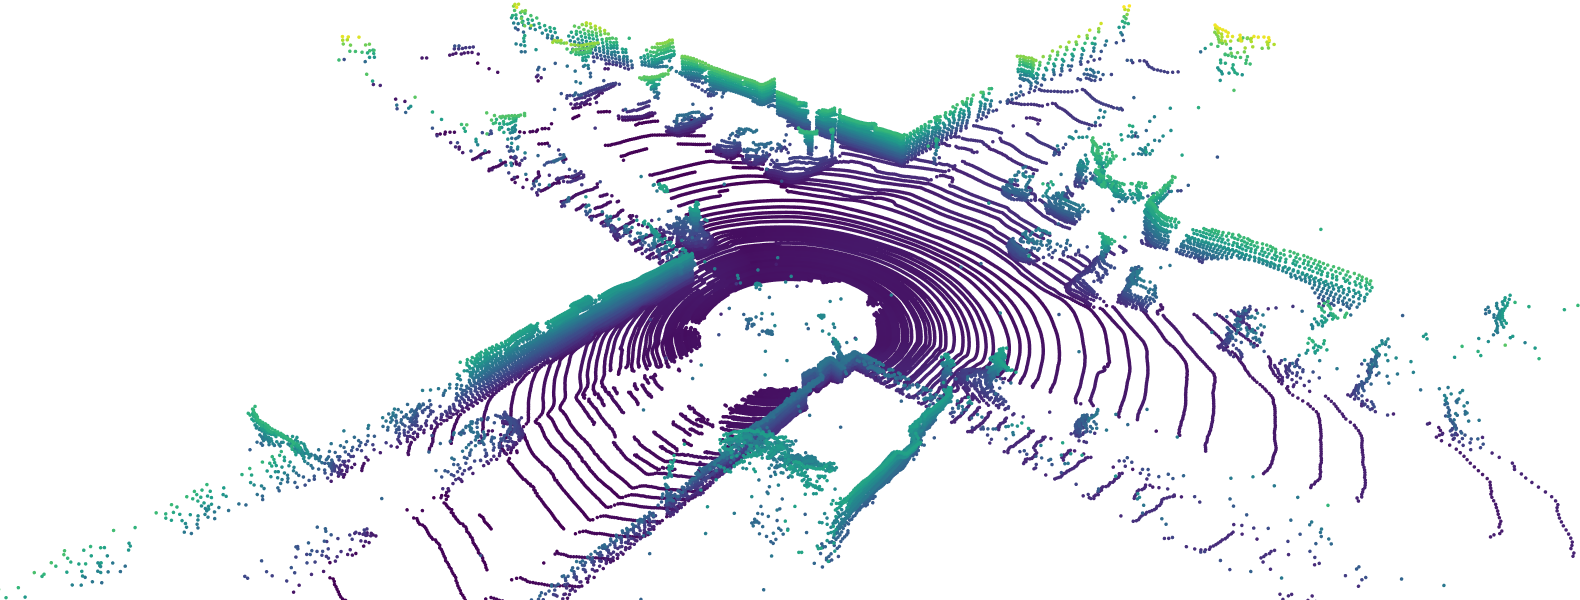
\includegraphics[width=\linewidth]{figures/qualitative/q2.png}
%     \end{minipage}
%     \begin{minipage}{0.24\textwidth}
%     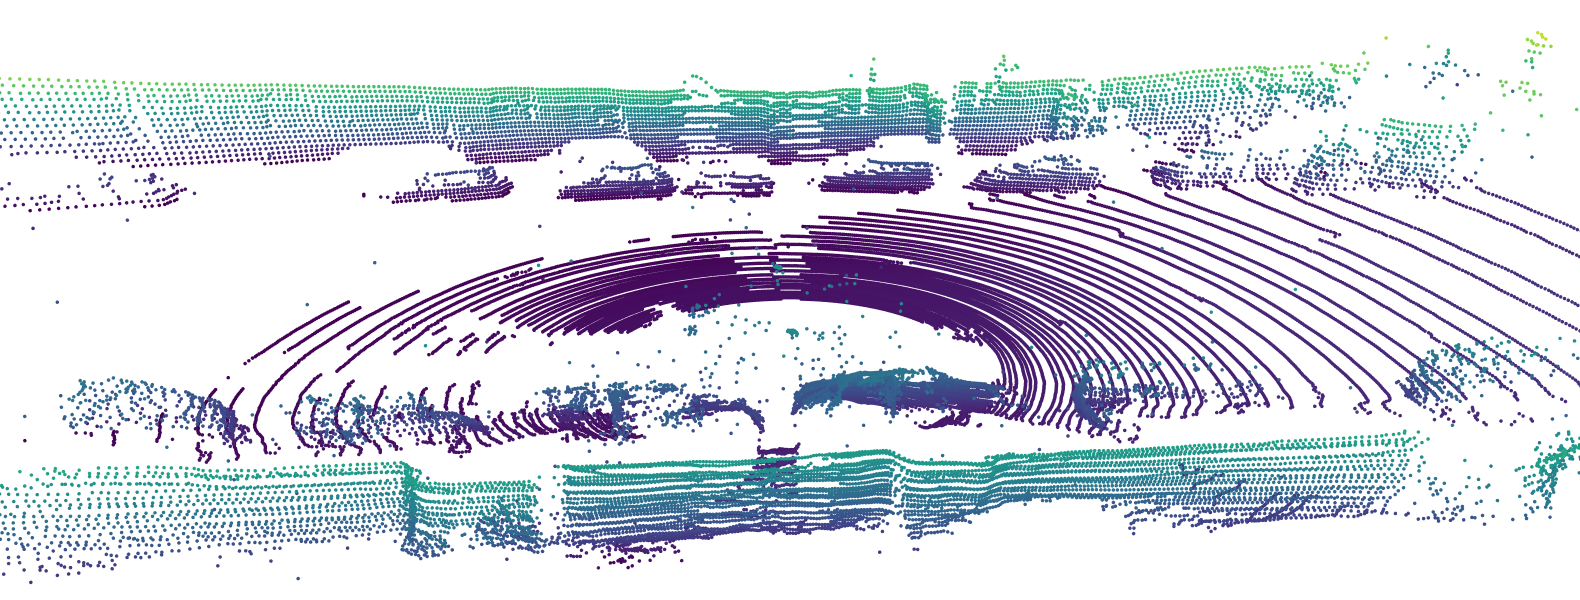
\includegraphics[width=\linewidth]{figures/qualitative/q3.png}
%     \end{minipage}
%     \begin{minipage}{0.24\textwidth}
%     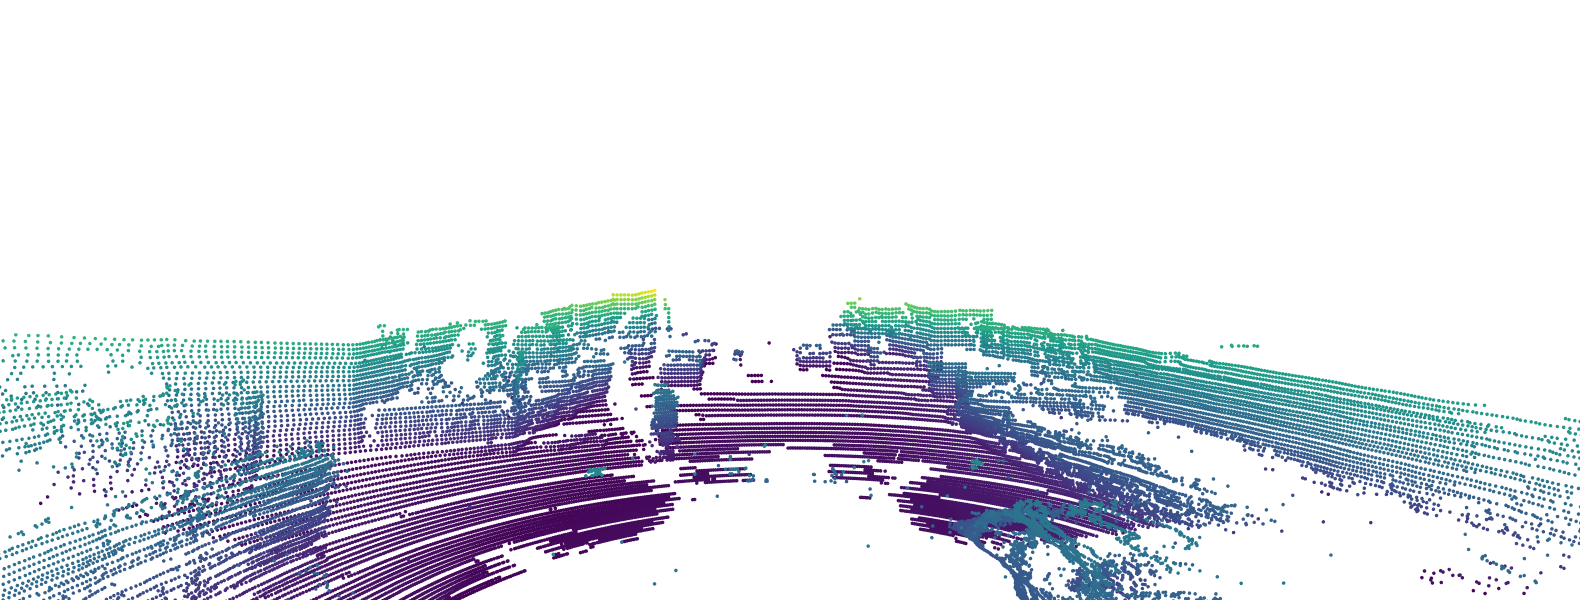
\includegraphics[width=\linewidth]{figures/qualitative/q4.png}
%     \end{minipage}
%     \caption{\textbf{Qualitative samples from \ours.}
%     We generate diverse scenes with cars, pedestrians and cyclist while faithfully capturing the LiDAR pattern. }
%     \label{fig:ours_qual}
% \end{figure*}

\begin{figure*}[t]
    \centering
    \begin{minipage}{0.24\textwidth}
        \begin{tikzpicture}
            \node[anchor=south west, inner sep=0] (img1) at (0,0) 
                {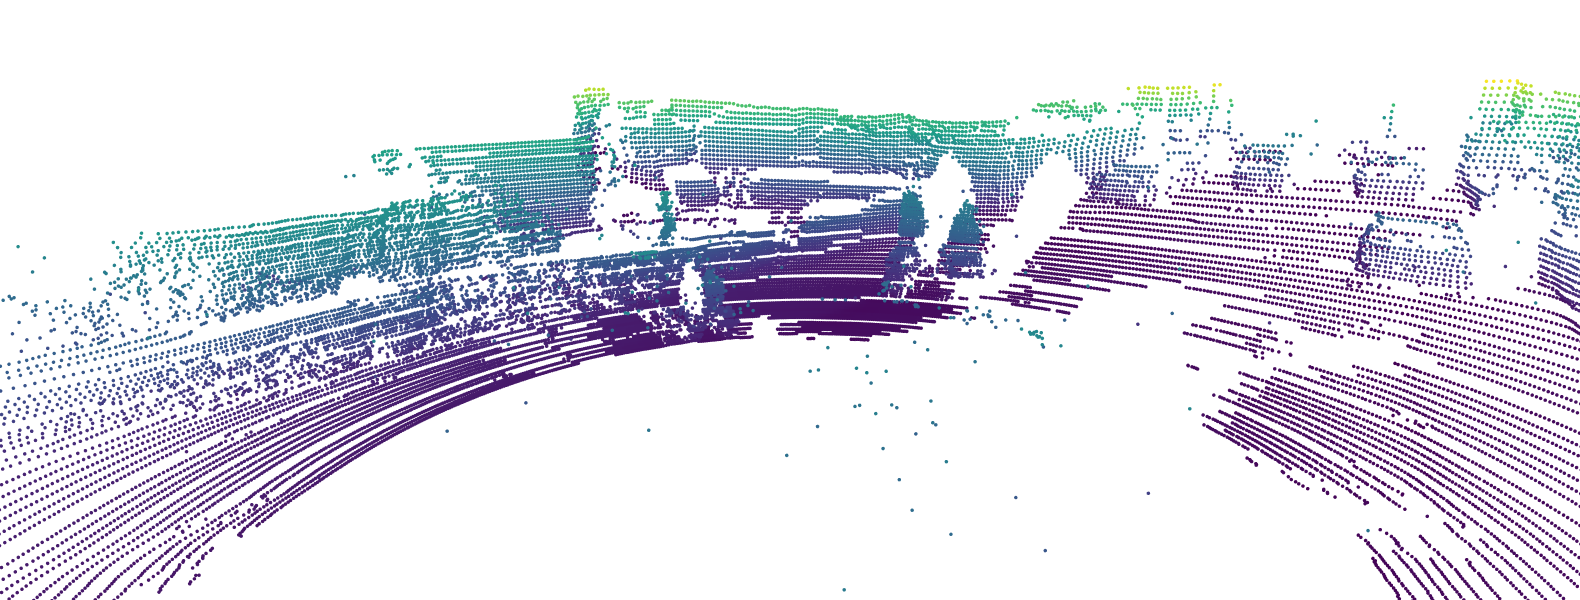
\includegraphics[width=\linewidth]{figures/qualitative/q1.png}};
            \begin{scope}[x={(img1.south east)},y={(img1.north west)}]
                % Adjust (x, y) coordinates from 0 to 1
                \draw[red, thick] (0.45, 0.49) circle (4pt); 
                \draw[red, thick] (0.59, 0.59) circle (5pt); 
            \end{scope}
        \end{tikzpicture}
    \end{minipage}
    \hfill
    \begin{minipage}{0.24\textwidth}
        \begin{tikzpicture}
            \node[anchor=south west, inner sep=0] (img2) at (0,0) 
                {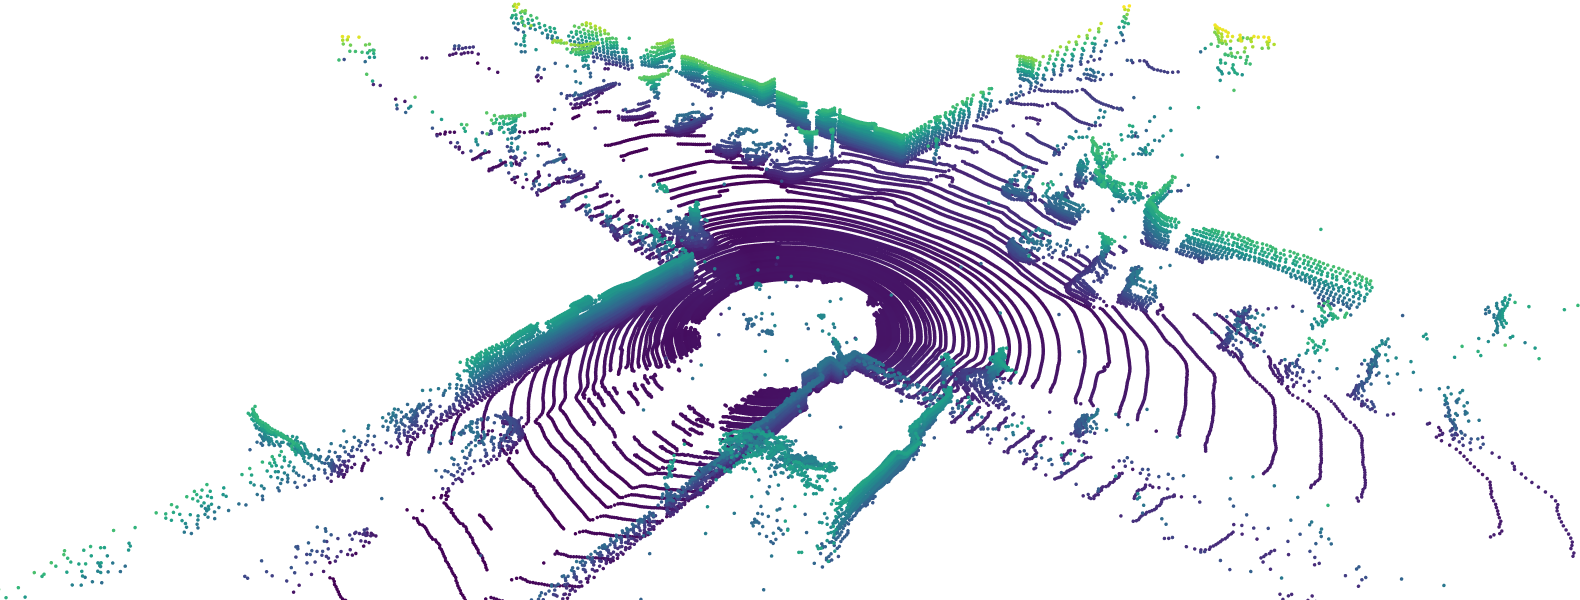
\includegraphics[width=\linewidth]{figures/qualitative/q2.png}};
            \begin{scope}[x={(img2.south east)},y={(img2.north west)}]
                % \draw[blue, thick] (0.3, 0.7) circle (0.1);
            \end{scope}
        \end{tikzpicture}
    \end{minipage}
    \hfill
    \begin{minipage}{0.24\textwidth}
        \begin{tikzpicture}
            \node[anchor=south west, inner sep=0] (img3) at (0,0) 
                {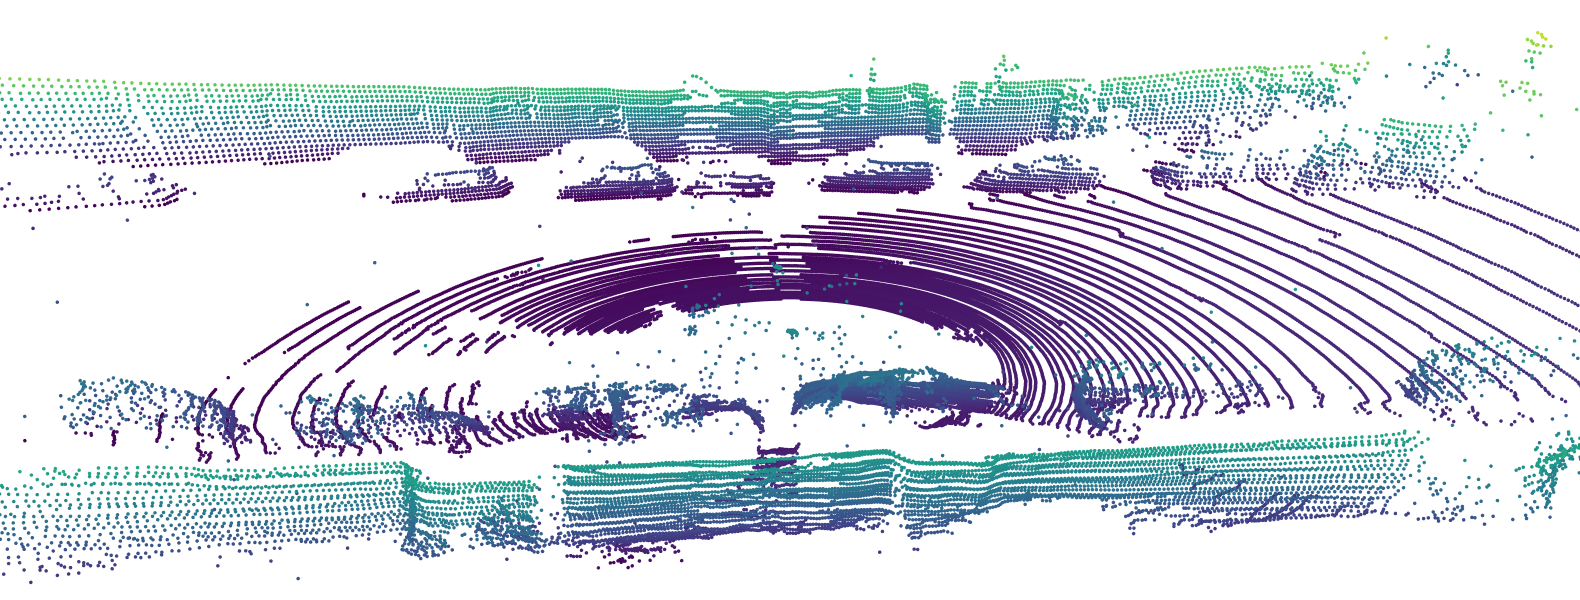
\includegraphics[width=\linewidth]{figures/qualitative/q3.png}};
            \begin{scope}[x={(img3.south east)},y={(img3.north west)}]
                % \draw[blue, thick] (0.6, 0.2) circle (0.1);
            \end{scope}
        \end{tikzpicture}
    \end{minipage}
    \hfill
    \begin{minipage}{0.24\textwidth}
        \begin{tikzpicture}
            \node[anchor=south west, inner sep=0] (img4) at (0,0) 
                {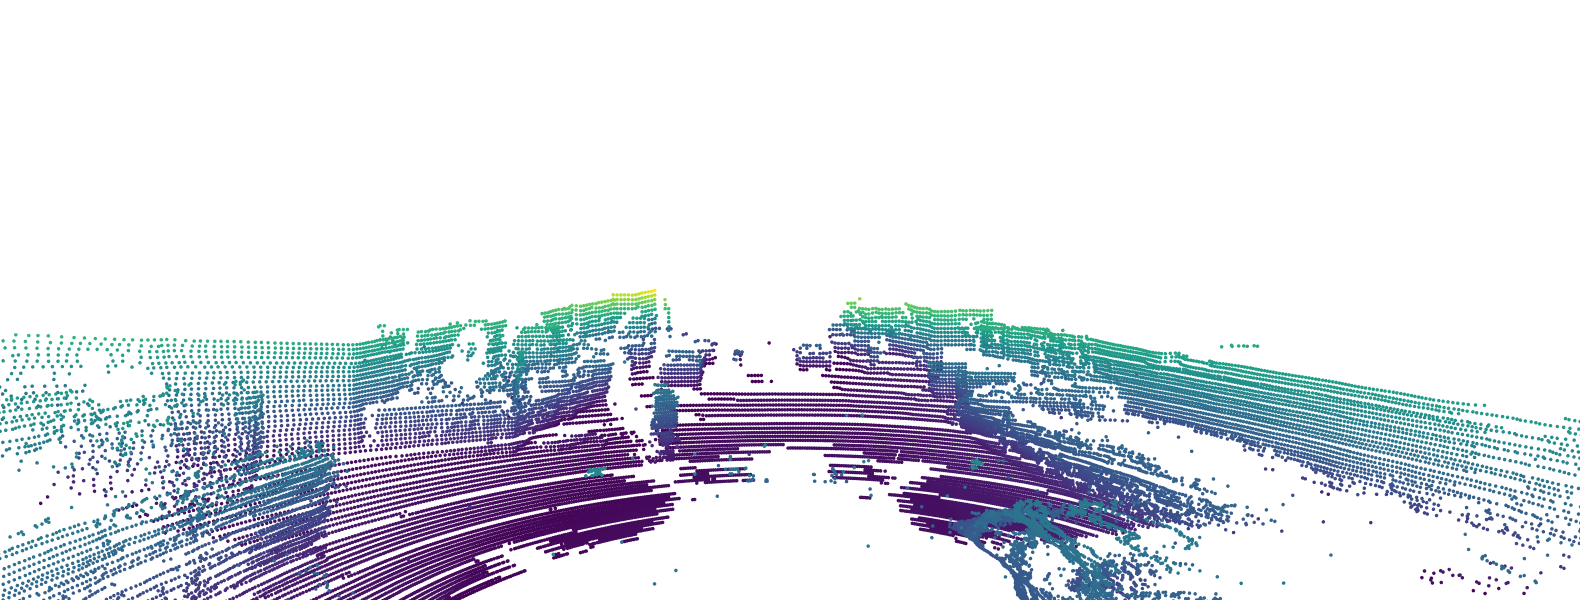
\includegraphics[width=\linewidth]{figures/qualitative/q4.png}};
            \begin{scope}[x={(img4.south east)},y={(img4.north west)}]
                \draw[red, thick] (0.42, 0.3) circle (4pt);
            \end{scope}
        \end{tikzpicture}
    \end{minipage}
    \caption{\textbf{Qualitative samples from \ours.}
    We generate diverse scenes with cars, pedestrians and cyclist while faithfully capturing the LiDAR pattern. }
    \label{fig:ours_qual}
\end{figure*}
%%%%%%%%%%%%%%%%%%%%%%



We compare our method against SOTA scene generation methods. We generate samples using a comparable number of steps: 250 for LiDM~\cite{ran_towards_2024} and 256 for R2DM~\cite{nakashima_lidar_2024} and R2Flow~\cite{nakashima_fast_2025}, following their official repositories. For fairness, we also use 256 steps for our model. For UltraLiDAR \cite{xiong_ultralidar_2023}, we use the publicly available samples released online. We generate our samples following \cite{ma_sit_2024} using the stochastic differential equation with the Euler-Maruyama solver.

To ensure a fair comparison, we follow~\cite{nakashima_fast_2025} and train LiDM \cite{ran_towards_2024} with a learnable absolute positional encoding inserted after the first UNet convolution.
This stabilizes orientation in generated scenes, allowing evaluation with non-rotation-invariant metrics (i.e. JSD, MMD) and improving performance on rotation-invariant metrics.

For each method, we generate 10,000 samples and evaluate them against the full dataset of real scenes (train-val evaluation), as is common in generative modeling \cite{nakashima_fast_2025}. 
For completeness, we also report results evaluated against the validation set (val-only evaluation).
For MMD, which requires computing the expensive Chamfer distance between all pairs of point clouds, we use 2,000 generated samples and evaluate them against 1,000 validation scenes, as in \cite{ran_towards_2024}.
The VAE alignment and end-to-end training require 48h and 70h, respectively, using 8 NVIDIA A100 GPUs.  \ours achieves an average inference speed of 0.6 s/scene, generating 10k samples in 1.45h on a single A100 with a batch size of 64.

We present quantitative results in Table~\ref{tab:sota} and qualitative comparisons in Figure~\ref{fig:qual}. For range-image metrics, \ours performs on par with the state of the art on FRID, while achieving a significant improvement on the FLD metric. For point-based metrics, which are particularly important given the ultimate goal of generating high-quality, realistic point clouds, our method surpasses previous approaches.
On bird’s-eye-view metrics, \ours improves the JSD score while achieving performance comparable to the state of the art on MMD.
Importantly, we achieve strong performance across both point and range metrics while other works show higher variance. We suspect that \cite{xiong_ultralidar_2023}'s low score likely results from its voxel-based architecture.
We present further qualitative results from our model in Figure \ref{fig:ours_qual}.

\begin{table}[htbp]
\caption{Effect of RGB Image Pretrained Priors and VAE Alignment.}
\vspace{-0.2cm}
\centering
\small
\resizebox{\linewidth}{!}{%
\begin{tabular}{ccccccccc}
\toprule

 
 \multicolumn{1}{c}{\rotatebox{0}{\textbf{RGB}}}   
 & \multicolumn{1}{c}{\textbf{VAE}}  
 & \multicolumn{1}{c}{\textbf{FRID}}    
 & \multicolumn{1}{c}{\textbf{FLD}}  
 & \multicolumn{1}{c}{\textbf{FSVD}}  
 & \multicolumn{1}{c}{\textbf{FPVD}}  
 & \multicolumn{1}{c}{\textbf{JSD}}    

 & \multicolumn{1}{c}{\textbf{MMD}}  
 \\
\textbf{Priors}  & \textbf{Align.} & {\footnotesize $\times 10^{0}$} & {\footnotesize $\times 10^{-1}$} & 
{\footnotesize $\times 10^{0}$} & {\footnotesize $\times 10^{0}$} & {\footnotesize$\times 10^{-2}$} &  {\footnotesize $\times 10^{-5}$}\\
 \midrule
\xmark & \xmark  & 13.44 & 4.98 & 9.97 & 11.21 & 5.08 &   8.99 \\
\cmark & \xmark &   12.81 & 4.52 & 10.13 & 11.39 & 4.98 &   8.87  \\
\cmark & \cmark &  \textbf{7.12} & \textbf{3.26} & \textbf{8.55} & \textbf{10.37 }& \textbf{4.70 }&   \textbf{8.76} \\
\bottomrule
\end{tabular}
}
\label{tab:abl_vae} 

\begin{tablenotes}[para]
    %\item 
    \footnotesize Direct use of RGB priors does not improve performance, whereas VAE alignment yields improvements across all metrics. 
\end{tablenotes}
\end{table}


\subsection{Ablations}

For faster experimentation in ablation studies, we first train the VAE from scratch for 400k steps during the alignment stage, and then perform end-to-end training of both the VAE and SiT for another 400k steps.
All ablation results are reported under the train-val evaluation setting.

\textbf{Effect of RGB Priors and VAE Alignment.} 
In this series of ablation experiments, we evaluate the impact of (i) leveraging priors from a backbone pretrained on a large-scale image dataset and (ii) incorporating our proposed VAE alignment step to better transfer these priors. To this end, we consider three settings: 

\begin{enumerate} 
    \item A base model where the VAE is trained from scratch in the first stage; then by keeping the VAE frozen the SiT is trained from scratch with random initialization in the second stage. 
    \item  The same as (1), except in the second stage SiT is initialized with RGB image pretrained weights instead of random initialization.
    \item VAE alignment is first applied by training the VAE from scratch to adapt it to pretrained RGB image priors; in the second stage, the VAE is kept frozen and SiT is trained, initialized with RGB image pretrained weights.
\end{enumerate} 

We note that these experiments do not employ end-to-end training. Instead, we follow the classical two-stage paradigm as in~\cite{ran_towards_2024,hu_rangeldm_2024}, where the VAE is first trained independently and then kept frozen during the second stage while training the FM model.

As shown in Table~\ref{tab:abl_vae}, using RGB priors alone does not improve performance, whereas the VAE alignment step leads to consistent improvements across all metrics. We conclude that the VAE alignment step reduces the gap with respect to the ImageNet-trained SiT input space, enabling more effective use of RGB prior knowledge. 

\begin{figure*}[ht]
\centering
% ===== Row: Car 1 =====
\begin{tabular}{lcc}
  \centering
  % left: stacked range images
\raisebox{5mm}{\multirow{1}{*}{\rotatebox[origin=c]{90}{\footnotesize GT}}} & 
\includegraphics[width=0.46\linewidth]{figures/car1/r3dpa_inpainting_gt_1_cropped_v3.pdf} & 
\includegraphics[width=0.46\linewidth]{figures/car2/r3dpa_inpainting_gt_2_cropped.pdf}\\ 
  
% \small \shortstack{Gen \\ RI} & 
\raisebox{5mm}{\multirow{1}{*}{\rotatebox[origin=c]{90}{ \footnotesize Gen}}} & 
\includegraphics[width=0.46\linewidth]{figures/car1/r3dpa_inpainting_gen_1_cropped_v3.pdf} & 
\includegraphics[width=0.46\linewidth]{figures/car2/r3dpa_inpainting_gen_2_cropped.pdf} \\
    
& \cropcenter{0.22\linewidth}{\detokenize{figures/car1/gt.png}}  \cropcenter{0.22\linewidth}{\detokenize{figures/car1/gen.png}} & 
\cropcenter{0.22\linewidth}{\detokenize{figures/car2/gt.png}}
\cropcenter{0.22\linewidth}{\detokenize{figures/car2/gen.png}} \\
& \footnotesize GT PC {~~~~~~~~~~~~~~~~~~~~~~~~~~~~~} \footnotesize Gen PC & \footnotesize GT PC  {~~~~~~~~~~~~~~~~~~~~~~~~~~~~~}  \footnotesize Gen PC   \\


\end{tabular}
\caption{\textbf{Test-time conditioning with 3D representations for object inpainting.} A user-specified mask (red) is drawn on top of the ground truth range image (center-cropped for visibility). The real scene is transported to the Gaussian distribution, then the user defined area is filled with noise. During the denoising process only the masked area is supervised with features corresponding to the target object class. The scenes are also presented projected to 3D points, colored according to the intersection with the frustum of the projected mask.}
\label{fig:inpaint}
\vspace{-0.2cm}
\end{figure*}
\begin{table}[htbp]
\caption{3D Representation Alignment and End-to-end Training.}
\vspace{-0.2cm}
\centering
\small
\resizebox{\linewidth}{!}{%
\begin{tabular}{ccccccc}
\toprule
 \multicolumn{1}{c}{\textbf{2nd Stage}}  
 & \multicolumn{1}{c}{\textbf{FRID}}    
 & \multicolumn{1}{c}{\textbf{FLD}}  
 & \multicolumn{1}{c}{\textbf{FSVD}}  
 & \multicolumn{1}{c}{\textbf{FPVD}}  
 & \multicolumn{1}{c}{\textbf{JSD}}   

 & \multicolumn{1}{c}{\textbf{MMD}}  
  \\
 \textbf{Alignment} & {\footnotesize $\times 10^{0}$} & {\footnotesize $\times 10^{-1}$} & 
{\footnotesize $\times 10^{0}$} & {\footnotesize $\times 10^{0}$} & {\footnotesize$\times 10^{-2}$} &  {\footnotesize $\times 10^{-5}$}\\
 \midrule
 No       & 7.12 & 3.26 & 8.55 & 10.37 & 4.70 &   8.76 \\
 Vanilla  & 7.23 & 3.28 & 8.52 & 10.25 & 4.64 & 8.81 \\
 Joint    & \textbf{4.14} & \textbf{2.23} & \textbf{7.96} & \textbf{9.69} & \textbf{4.55} &  \textbf{8.41} \\
\bottomrule
\end{tabular}
}
\hspace{-0.3cm}
\begin{tablenotes}[para]
    \footnotesize 
     We first perform the VAE alignment step and use its weights in the subsequent experiments. \textit{No alignment:} the VAE is kept frozen and SiT is trained with RGB image pretrained weights. \textit{Vanilla alignment:} the VAE is kept frozen and 3D representation guidance is propagated to the flow model. \textit{Joint alignment:} end-to-end training with 3D guidance propagated to both the flow model and the VAE encoder.
\end{tablenotes}
\label{tab:abl_repas}
\end{table}


\textbf{Effect of 3D Alignment and End-to-end Training.}
In this series of experiments, we study the impact of 3D representation alignment and end-to-end training. 
In the previous section, we leveraged RGB priors from pretrained models by first performing VAE alignment and then, in a second stage, freezing the VAE while training the FM model SiT initialized with RGB image pretrained weights. Since this setting does not incorporate any guidance from 3D representations during second stage, we refer to it as \textit{no alignment}. 
The next experiment, \textit{vanilla alignment}, also keeps the VAE frozen but propagates 3D representation guidance only to the FM model. 
Finally, \textit{joint alignment} corresponds to our end-to-end training setup, where 3D representation guidance is propagated to both the FM model and the VAE encoder.

Table~\ref{tab:abl_repas} shows that end-to-end training with 3D representations substantially improves generation quality across all metrics.

%%%%%%%%%%%%%%%%%%%%%%%%%%%%%%%%%% ONLY TRAIN-VAL RESULTS
\begin{table}[t]
\caption{Comparison of UNet and SiT.}
\vspace{-0.2cm}
\label{tab:abl_arch}
\centering
\small
\resizebox{\linewidth}{!}{%
\begin{tabular}{ccccccc}
\toprule
  \multirow{2}{*}{\textbf{Backbone}}   
 & \multicolumn{1}{c}{\textbf{FRID}}    
 & \multicolumn{1}{c}{\textbf{FLD}}  
 & \multicolumn{1}{c}{\textbf{FSVD}}  
 & \multicolumn{1}{c}{\textbf{FPVD}}  
 & \multicolumn{1}{c}{\textbf{JSD}}    
 % & \multicolumn{1}{c}{\textbf{TV}} 
 & \multicolumn{1}{c}{\textbf{MMD}}  
 \\
  &  {\footnotesize $\times 10^{0}$} & {\footnotesize $\times 10^{-1}$} & 
{\footnotesize $\times 10^{0}$} & {\footnotesize $\times 10^{0}$} & {\footnotesize$\times 10^{-2}$}  & {\footnotesize $\times 10^{-5}$}\\
 \midrule
UNet of \cite{ran_towards_2024}   &  7.70 & \textbf{3.09} & \textbf{7.80} & 9.61 & 4.64   & \textbf{8.83}  \\ 
SiT-B/2 &  \textbf{6.08} & 3.17 & 7.89 & \textbf{8.86} & \textbf{4.52} & 8.95 \\

\bottomrule

\end{tabular}
}

\begin{tablenotes}[para]
    \footnotesize
    \hspace{-0.2cm} SiT achieves comparable or better results with twice fewer parameters.
\end{tablenotes}
\vspace{-0.5cm}

\end{table}


\textbf{Comparison of UNet and SiT.} UNet is one of the most widely used architectures for implementing diffusion and FM models~\cite{ran_towards_2024,nakashima_lidar_2024, zyrianov2022learning,hu_rangeldm_2024}. 
To provide a comparison with SiT, we use the UNet architecture from LiDM~\cite{ran_towards_2024}. Following~\cite{tian_u-repa_2025}, we supervise the representations of its middle block with projected ScaLR \cite{puy2024three} features for an end-to-end training \NS{without VAE Alignment step}.  
We note that UNet has roughly twice as many parameters as our SiT backbone (266M vs. 130M). 
Nevertheless, Table~\ref{tab:abl_arch} shows that SiT-B/2 achieves comparable or better results with fewer parameters.



\subsection{Test-Time Conditioning with 3D Representations}

We explore inference time guidance using the alignment loss without retraining.
Given a feature grid of a scene (such as Figure~\ref{fig:scalr_features}), generation can be guided toward consistency with these features by backpropagating the gradient of the alignment loss with respect to the latent vector $z_t$. 
The loss is computed between the SiT's internal representation and the conditional features, and combined with the SiT velocity vector to transport the latent toward a LiDAR scene matching the target features.  

We propose two applications of this representation conditioning: object in-painting (using diffusion inversion \cite{song2021denoising}) and scene mixing, where features from multiple real scenes are merged to produce a smooth combination (see Figure~\ref{fig:scene_edit}).
For object in-painting, we transport a real scene toward the Gaussian distribution using the ordinary differential equations defined by the SiT velocity field. 
Noise is added to the tokens within a user-defined mask, after which the process is reversed: denoising is applied starting from this noise while supervising the internal representations of the masked tokens with 3D features of the target object category. The object features are extracted via averaging over the target class on a single scene. The result is a reconstructed scene in which the masked region is filled with points that are both consistent with the surroundings and aligned with the conditioned object. Figure~\ref{fig:inpaint} presents qualitative examples of inpainting.
We note that, these two applications are presented as illustrative examples of the potential of our method, rather than as claims of state-of-the-art performance.

\begin{figure}[t!]
    \centering
    \begin{tabular}{ccc}
        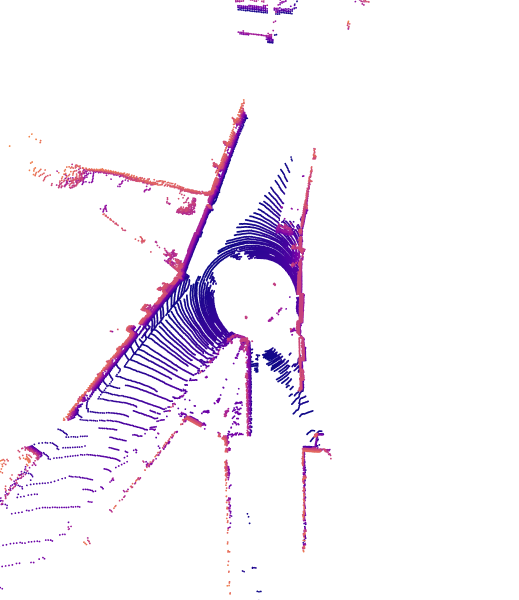
\includegraphics[width=0.29\columnwidth]{figures/mixing/mix_1.png} &
        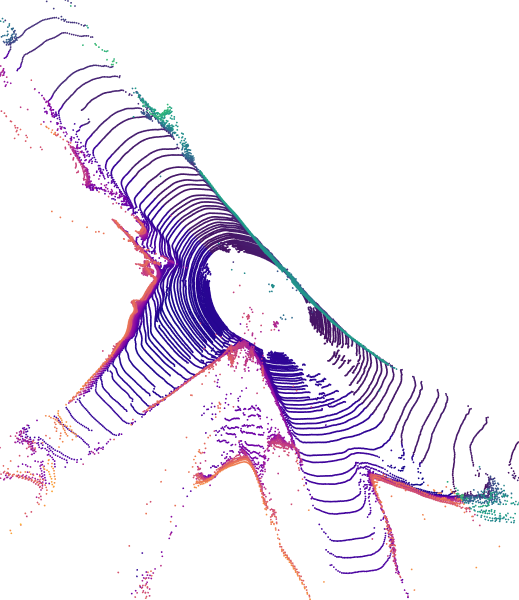
\includegraphics[width=0.29\columnwidth]{figures/mixing/mix_2.png} &
        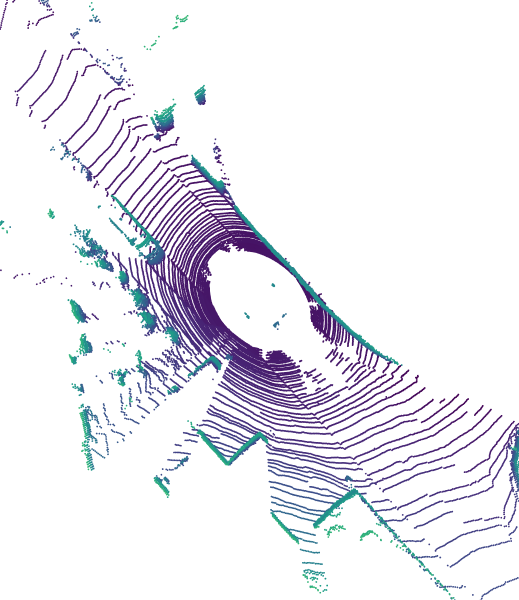
\includegraphics[width=0.29\columnwidth]{figures/mixing/mix_3.png} \\
        {\footnotesize Real scene - I}   & \footnotesize Generated scene & \footnotesize Real scene - II \\
    \end{tabular}
    \caption{\textbf{Test-time conditioning with 3D representations for scene mixing.} We condition on stitched features from two real scenes, mixing the left half of one scene with the right half of the other. Generated scene (middle) mixes layouts from real scenes: the left part (purple) resembles the first real scene (left), while the right part (green) resembles the second real scene (right). }
    \label{fig:scene_edit}
    \vspace{-0.5cm}
\end{figure}